\documentclass{letter}
\usepackage[parfill]{parskip}

\usepackage{hyperref}

\usepackage{tikz}
\usetikzlibrary{arrows.meta}
\renewcommand{\familydefault}{\sfdefault}

\begin{document}
\begin{center}
\textbf{COMP3700 Activity 5}\\
Tripp Isbell\\
cai0004@auburn.edu
\end{center}

\begin{enumerate}
	\item Identify entities
	\begin{itemize}
		\item Customers
		\begin{itemize}
			\item name
			\item ID
			\item email
			\item payment method
			\item purchase history
		\end{itemize}
		\item Products
		\begin{itemize}
			\item product ID
			\item price
			\item inventory count
			\item transaction history
		\end{itemize}
		\item Employees
		\begin{itemize}
			\item employee ID
			\item wage
			\item schedule
			\item rank or privilege level
			\item name
		\end{itemize}
		\item Suppliers
		\begin{itemize}
			\item supplier ID
			\item name
			\item products available
			\item price of products
		\end{itemize}
	\end{itemize}
\newpage
	\item Identify relationships
	\begin{itemize}
		\item Customers $\longrightarrow$ name (one-to-one)
		\item Customers $\longrightarrow$ customer ID (one-to-one)
		\item Customers $\longrightarrow$ email (one-to-one)
		\item Customers $\longrightarrow$ payment method (one-to-many)
		\item Customers $\longrightarrow$ purchase history (one-to-many) (technically one-to-list)
		\item Customers $\longleftrightarrow$ Products (many-to-many)
		\item Products $\longrightarrow$ product ID (one-to-one)
		\item Products $\longrightarrow$ price (one-to-one)
		\item Products $\longrightarrow$ quantity (one-to-one)
		\item Products $\longrightarrow$ transaction history 
		\item Products $\longleftrightarrow$ Suppliers (many-to-many)
		\item Suppliers $\longrightarrow$ prices (one-to-many)
		\item Suppliers $\longrightarrow$ supplier ID (one-to-one)
		\item Suppliers $\longrightarrow$ name (one-to-one)
		\item Suppliers $\longleftrightarrow$ Employees (management)
		\item Employees $\longrightarrow$ employee ID (one-to-one)
		\item Employees $\longrightarrow$ wage (one-to-one)
		\item Employees $\longrightarrow$ schedule (one-to-one)
		\item Employees $\longrightarrow$ rank (one-to-one)
		\item Employees $\longrightarrow$ name (one-to-one)
	\end{itemize}
\newpage
	\item Draw entity-relationship diagram\\
	
	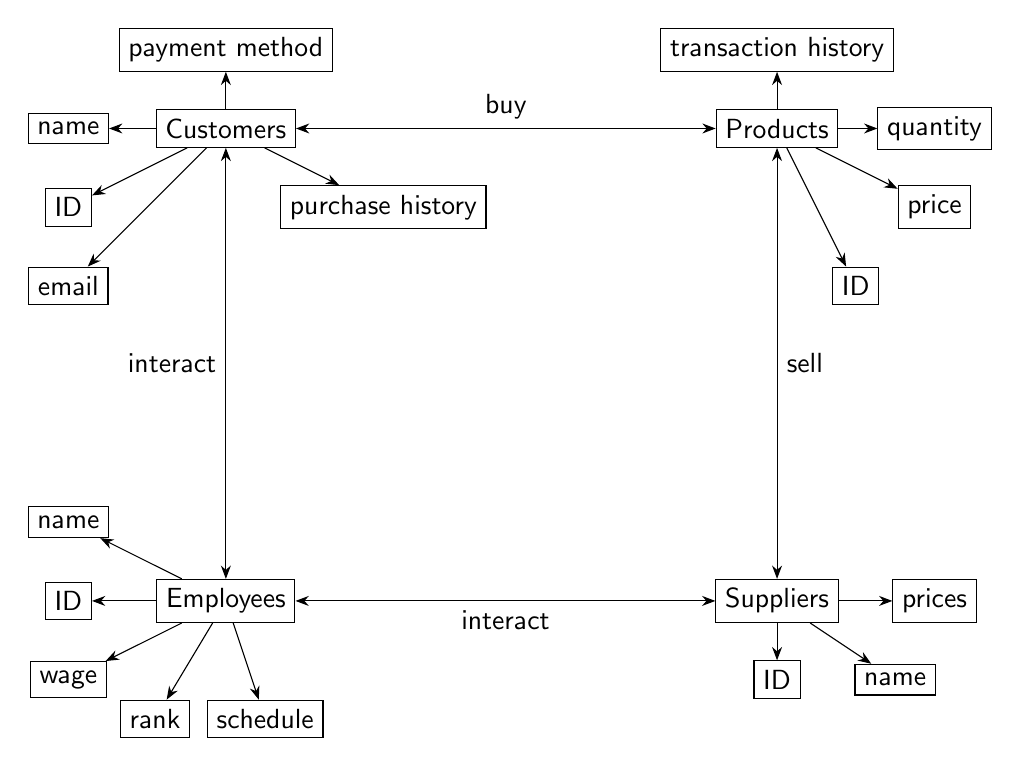
\begin{tikzpicture}[scale=1]
	\begin{scope}[every node/.style={rectangle,draw}, every label/.append style={font=\scriptsize}]
		\node (Customers) at (1, 8) {Customers};
			\node (Customer name) at (-1,8) {name};
			\node (Customer ID) at (-1,7) {ID};
			\node (Customer email) at (-1,6) {email};
			\node (Customer payment method) at (1,9) {payment method};
			\node (Customer purchase history) at (3,7) {purchase history};
		\node (Employees) at (1, 2) {Employees};
			\node (Employee ID) at (-1, 2) {ID};
			\node (Employee name) at (-1,3) {name};
			\node (Employee wage) at (-1,1) {wage};
			\node (Employee rank) at (0.1, 0.5) {rank};
			\node (Employee schedule) at (1.5,0.5) {schedule};
		\node (Products) at (8, 8) {Products};
			\node (Product ID) at (9,6) {ID};
			\node (Product price) at (10,7) {price};
			\node (Product quantity) at (10,8) {quantity};
			\node (Product transaction history) at (8,9) {transaction history};
		\node (Suppliers) at (8,2) {Suppliers};
			\node (Supplier prices) at (10,2) {prices};
			\node (Supplier ID) at (8,1) {ID};
			\node (Supplier name) at (9.5,1) {name};
	\end{scope}
	\begin{scope}[>={Stealth[black]}]
	\path [->] (Customers) edge (Customer name);
	\path [->] (Customers) edge (Customer ID);
	\path [->] (Customers) edge (Customer email);
	\path [->] (Customers) edge (Customer payment method);
	\path [->] (Customers) edge (Customer purchase history);
	\path [<->] (Customers) edge node[above] {buy} (Products);
	
	\path [->] (Products) edge (Product ID);
	\path [->] (Products) edge (Product price);
	\path [->] (Products) edge (Product quantity);
	\path [->] (Products) edge (Product transaction history);
	\path [<->]  (Products) edge node[right] {sell} (Suppliers);
	
	\path [->] (Suppliers) edge (Supplier prices);
	\path [->] (Suppliers) edge (Supplier ID);
	\path [->] (Suppliers) edge (Supplier name);
	\path [<->] (Suppliers) edge node[below] {interact} (Employees);
	
	\path [->] (Employees) edge (Employee ID);
	\path [->] (Employees) edge (Employee name);
	\path [->] (Employees) edge (Employee wage);
	\path [->] (Employees) edge (Employee rank);
	\path [->] (Employees) edge (Employee schedule);
	\path [<->] (Employees) edge node[left] {interact} (Customers);
	\end{scope}
	\end{tikzpicture}
\end{enumerate}

\end{document}